\section{nasm}
\label{tool:nasm}

\href{https://nasm.us/}{Netwide Assembler (NASM)}, is  asssembler for the x86
CPU architecture portable to nearly every modern platform, and with code
generation for many platforms old and new.

\subsection*{nasm Assembly File Structure}

In this section, we'll go through the basic structure of an Assembly file, and
in the following two sections, we will cover assembling it and debugging it. We
will be working on a template {\bf Hello World! } Assembly code as a sample, to
first learn the general structure of an assembly file and then how to assemble
it and debug it. Let us start by taking a look at and dissecting a sample Hello
World! Assembly code template:
\begin{verbatim}
         global  _start

         section .data
message: db      "Hello!"

         section .text
_start:
         mov     rax, 1
         mov     rdi, 1
         mov     rsi, message
         mov     rdx, 18
         syscall

         mov     rax, 60
         mov     rdi, 0
         syscall
\end{verbatim}

This Assembly code (once assembled and linked) should print the string 'Hello!'
to the screen. We won't go into detail on how this is processed just yet, but
we need to understand the main elements of the code template.


 \begin{figure}
  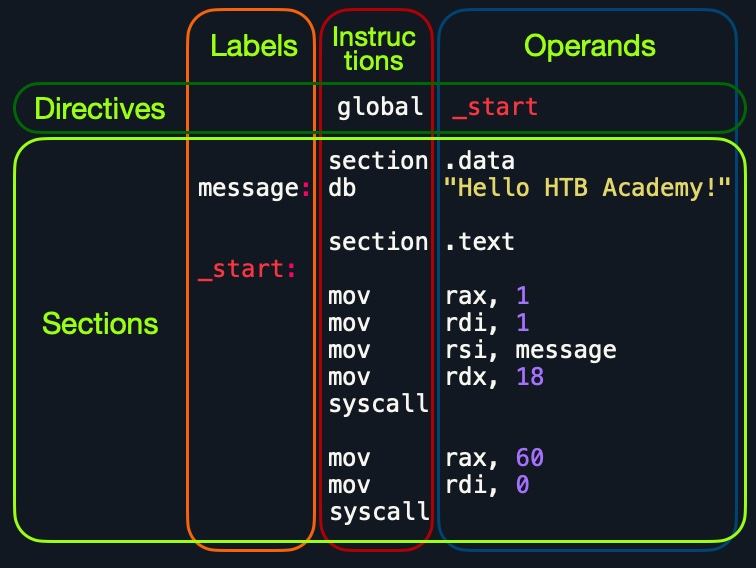
\includegraphics[width=\linewidth]{tools/all/images/nasm_structure.jpg}
  \caption{nasm structure}
  \label{fig:nasm_structure}
\end{figure}

Each label can be referred to by instructions or by directives.

The code is composed of three main parts:
\begin{verbatim}
Section 	    Description
global _start 	This is a directive that directs the code to start executing 
                at the _start label defined below.
section .data 	This is the data section, which should contain all of the variables.
section .text 	This is the text section containing all of the code to be executed.
\end{verbatim}

Both the \verb+.data+ and \verb+.text+ sections refer to the data and text
memory segments, in which these instructions will be stored.


\subsubsection*{Directives}

An Assembly code is line-based, which means that the file is processed
line-by-line, executing the instruction of each line. We see at the first line
a directive \verb+global _start+, which instructs the machine to start
processing the instructions after the \verb+_start+ label. So, the machine goes
to the \verb+_start+ label and starts executing the instructions there, which
will print the message on the screen. This will be covered more thoroughly in
the Control Instructions sections.

\verb+extern <funcname_1>, <funcname_2>+ is used to declare external functions
that will be linked later

\subsubsection*{Variables}

Next, we have the \verb+.data+ section. The data section holds our variables to
make it easier for to define variables and reuse them without writing them
multiple times. Once we run the program, all of variables will be loaded into
memory in the data segment.

We can define variables using \verb+db+ for a list of bytes, \verb+dw+ for a
list of words, and so on. Variable  can be labeled  in order to be referenced.
The following are some examples of defining variables:
\begin{verbatim}
db 0x0a 	Defines the byte 0x0a, which is a new line.
message db 0x41, 0x42, 0x43, 0x0a 	Defines the label message => abc\n.
message db "Hello World!", 0x0a 	Defines the label message => Hello World!\n.
\end{verbatim}

Furthermore, we can use the \verb+equ+ instruction with the \verb+$+ token to evaluate an expression, like the length of a defined variable's string. 
\begin{verbatim}
section .data
    message db "Hello World!", 0x0a
    length  equ $-message
\end{verbatim}

\subsubsection*{Code}

The second (and most important) section is the \verb+.text+ section. This
section holds all of the assembly instructions and loads them to the text
memory segment. Once all instructions are loaded into the text segment, the
processor starts executing them one after another.

The default convention is to have the \verb+_start+ label at the beginning of
the \verb+.text+ section, which -as per the \verb+global _start+ directive-
starts the main code that will be executed as the program runs. As we will see
later in the module, we can define other labels within the .text section, for
loops and other functions.

The text segment within the memory is read-only. 

The data section, on the other hand, is read/write but not executable, so any
code we write to it cannot be executed. This separation is part of memory
protections to mitigate things like buffer overflows and other types of binary
exploitation.

With this, we should understand the basic structure of an Assembly file.


\section{Assembling \& Disassembling}

\subsubsection*{linux}
\begin{verbatim}
nasm -f elf64 helloWorld.s
ld -o helloWorld helloWorld.o
ld ${fiename}.o -o ${fileName} -lc --dynamic-linker /usr/lib/ld-linux-x86-64.so.2
\end{verbatim}

\begin{verbatim}
objdump -M intel -d helloWorld
\end{verbatim}


\subsubsection*{windows}
\url{https://sonictk.github.io/asm_tutorial/}


